\chapter{User Guide}

The AI model, backend, and frontend have been configured and deployed. To use the software, please download the \textit{Expo} app from the Google Play Store or Apple App Store, and then scan the QR code below.

\begin{figure}[!ht]
    \centering
    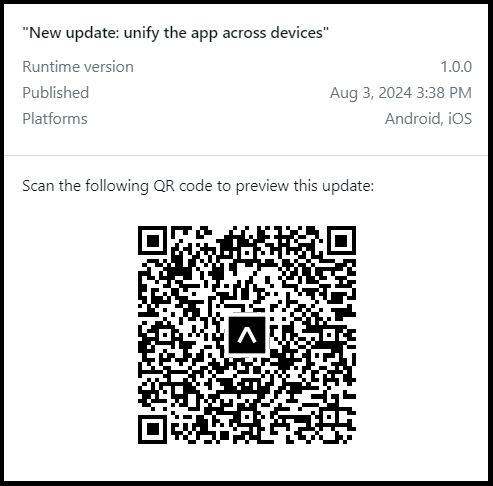
\includegraphics[width=0.5\linewidth]{LATEX/Appendices/Images/Software/deployed-app-qr-code.png}
    
    \label{fig:deployed-app-qr-codel}
\end{figure}

Alternatively, after installing the \textit{Expo} app, please click \href{https://expo.dev/preview/update?message=New\%20update\%3A\%20unify\%20the\%20app\%20across\%20devices&updateRuntimeVersion=1.0.0&createdAt=2024-08-03T14\%3A38\%3A52.572Z&slug=exp&projectId=032f6af8-bb36-47b5-80a0-f6f070705b75&group=e0b07c3c-0576-44ea-be88-aef4dbfc942a}{here}. This link will redirect you to the Expo app, where the software will be rendered.

If you would like to deploy the software yourself, either locally or globally, you can do this with \textit{Docker}, which has already been configured. For more information on commands to run, please read the \textit{README.md} files located in the root of the source code, in the \textit{ASACBackEnd} and \textit{ASACFrontEnd} directories.

Please note that the frontend was developed on iOS, so there may be discrepancies on Android. Additionally, to use the AI system, you need a \textit{.txt} file with a legal employment contract for the model. You can either create this file yourself or use the sample included in the source code under \textit{UsageFiles}.


